\documentclass[12pt]{article}
\usepackage[utf8]{inputenc}
\usepackage[T1]{fontenc}
\usepackage[french]{babel}
\usepackage{geometry}
\geometry{a4paper, margin=1in}
\usepackage{graphicx}
\usepackage{hyperref}
\usepackage{listings}
\usepackage{xcolor}
\usepackage{tikz}
\usetikzlibrary{positioning, arrows.meta, calc}
\usepackage{amsmath}
\usepackage{float}
\usepackage{subcaption}

% Configuration pour le code SQL et Python
\definecolor{codegreen}{rgb}{0,0.6,0}
\definecolor{codegray}{rgb}{0.5,0.5,0.5}
\definecolor{codepurple}{rgb}{0.58,0,0.82}
\definecolor{backcolour}{rgb}{0.95,0.95,0.92}

\lstdefinestyle{mystyle}{
    backgroundcolor=\color{backcolour},   
    commentstyle=\color{codegreen},
    keywordstyle=\color{magenta},
    numberstyle=\tiny\color{codegray},
    stringstyle=\color{codepurple},
    basicstyle=\ttfamily\footnotesize,
    breakatwhitespace=false,         
    breaklines=true,                 
    captionpos=b,                    
    keepspaces=true,                 
    numbers=left,                    
    numbersep=5pt,                  
    showspaces=false,                
    showstringspaces=false,
    showtabs=false,                  
    tabsize=2
}

\lstset{style=mystyle}

\begin{document}

\begin{titlepage}
    \centering
    \vspace*{4cm}
    
    {\huge \textbf{Rapport de Projet de Base de Données}} \\[1cm]
    
    {\Large Université Sorbonne Paris Nord} \\[0.5cm]
    {\large Licence 3 Informatique} \\[2cm]

    \textbf{\Large Sujet : Application de Streaming de Films} \\[2cm]

    \textbf{Membres du groupe :} \\[0.5cm]
    {\large Sanjai RAMALINGAME [12101328]} \\
    {\large Ismael BARRY [12109433]} \\
    {\large Kevin MADIVANANE [12107107]} \\[2cm]

    {\large Date : 1er Janvier 2026}
    
    \vfill
\end{titlepage}

\newpage
\tableofcontents
\newpage

\section{Introduction}

Dans le cadre de notre unité d'enseignement de Base de Données, nous avons conçu et développé une application nommée \textbf{"MyStream BDD"}. Il s'agit d'une plateforme d'exploration cinématographique permettant aux utilisateurs de rechercher, filtrer et consulter des informations détaillées sur une vaste collection de films.

L'objectif était double :
\begin{enumerate}
    \item \textbf{Modélisation et Gestion des Données :} Concevoir un schéma relationnel robuste (en respectant les formes normales) pour stocker efficacement les métadonnées de films (titres, genres, casting, équipe technique, notes, etc.).
    \item \textbf{Développement Applicatif :} Créer une interface utilisateur graphique (GUI) en Python capable d'interagir dynamiquement avec la base de données PostgreSQL pour offrir une expérience fluide.
\end{enumerate}

\subsection{Technologies Utilisées}
\begin{itemize}
    \item \textbf{Langage :} Python 3 pour la logique applicative.
    \item \textbf{SGBD :} PostgreSQL pour le stockage et la gestion des données.
    \item \textbf{Interface Graphique :} PyQt6 (Qt Widgets, Gui, Core) pour une interface moderne et réactive.
    \item \textbf{Connecteur :} \texttt{psycopg2} pour communiquer entre Python et PostgreSQL.
    \item \textbf{Réseau :} \texttt{requests} pour le chargement asynchrone des affiches de films depuis le web.
\end{itemize}

\subsection{Lancement de l'application}
Pour lancer l'application, il faut s'assurer d'avoir installé les dépendances (\texttt{PyQt6}, \texttt{psycopg2}, \texttt{requests}) et exécuter la commande suivante depuis la racine du projet :

\begin{lstlisting}[language=bash]
python3 Projet_SQL/stream_app.py
\end{lstlisting}

\newpage
\section{Fonctionnalités de l'Application}

Nous avons implémenté les fonctionnalités suivantes :

\subsection{Recherche et Filtrage Avancé}
L'utilisateur peut rechercher des films selon plusieurs critères combinables :
\begin{itemize}
    \item \textbf{Recherche textuelle :} Par titre de film ou par mot-clé associé.
    \item \textbf{Filtrage par Genre :} Sélection multiple via un menu déroulant (ex: Action, Comédie, Drame...).
    \item \textbf{Filtrage par Année :} Un double curseur (slider) permet de définir une plage d'années de sortie (ex: 2000 - 2020).
    \item \textbf{Filtrage par Note :} Un double curseur permet de filtrer les films selon leur note moyenne (ex: entre 7.5 et 10).
\end{itemize}

\begin{figure}[htbp]
    \centering
    \begin{subfigure}[t]{0.32\textwidth}
        \centering
        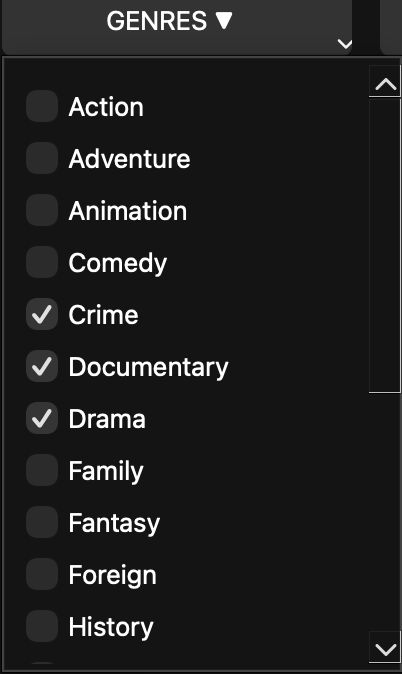
\includegraphics[width=\textwidth]{filtrage1.jpeg}
      
        \label{fig:filtrage1}
    \end{subfigure}
    \hfill % Espace flexible pour bien répartir les images
    \begin{subfigure}[t]{0.32\textwidth}
        \centering
        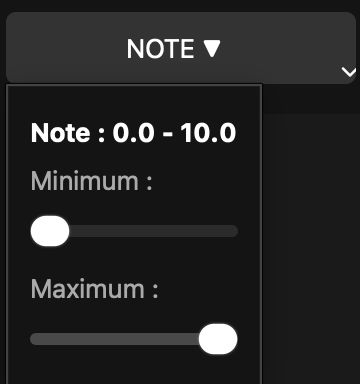
\includegraphics[width=\textwidth]{filtrage2.jpeg}
     
        \label{fig:filtrage2}
    \end{subfigure}
    \hfill
    \begin{subfigure}[t]{0.32\textwidth}
        \centering
        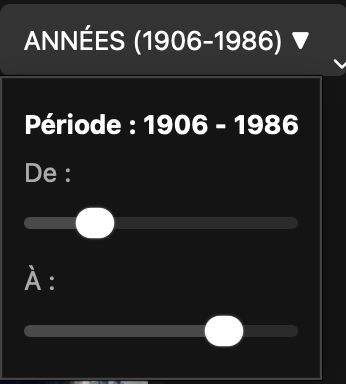
\includegraphics[width=\textwidth]{filtrage3.jpeg}
     
        \label{fig:filtrage3}
    \end{subfigure}
    
    \caption{Fonctionnalités de recherche et de filtrage avancé}
    \label{fig:recherche-filtrage}
\end{figure}



\subsection{Affichage et Navigation}
\begin{itemize}
    \item \textbf{Affichage sous forme de grille :} Les films sont présentés sous forme de "cartes" affichant l'affiche, le titre et la note.
    \item \textbf{Pagination :} Pour gérer le grand volume de données, les résultats sont paginés (40 films par page).
    \item \textbf{Chargement Asynchrone :} Les images (affiches) sont chargées dans des threads séparés (\texttt{QThread}) pour ne pas bloquer l'interface pendant le téléchargement.
\end{itemize}
\begin{figure}[H]
    \centering
    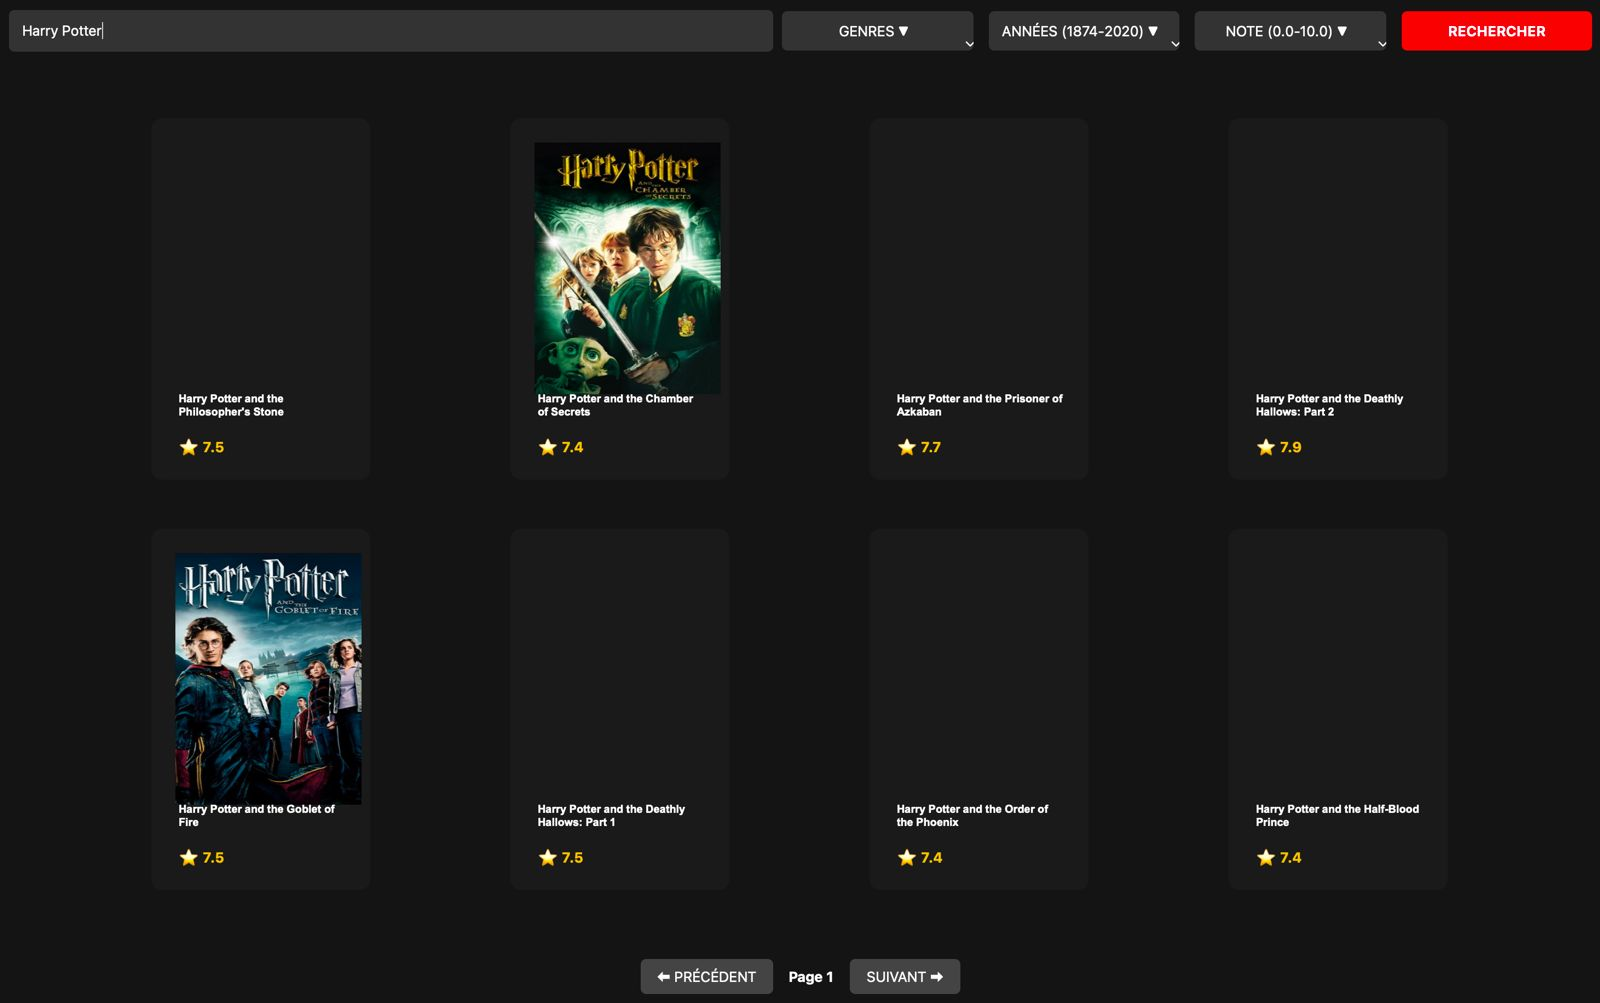
\includegraphics[width=0.75\linewidth]{affichage et navigation.jpeg}
    \caption{}
    \label{fig:placeholder1}
\end{figure}

\subsection{Vue Détaillée}
En cliquant sur un film, une fenêtre détaillée s'ouvre, affichant :
\begin{itemize}
    \item Le synopsis complet (\textit{overview}).
    \item Les métadonnées : Date de sortie, Durée, Langue originale, Note moyenne.
    \item \textbf{Casting :} Liste déroulante des acteurs principaux et leurs rôles.
    \item \textbf{Équipe Technique :} Liste déroulante des réalisateurs, scénaristes et producteurs.
\end{itemize}
\begin{figure}[H]
    \centering
    \includegraphics[width=0.40\linewidth]{vue detaillée.jpeg}
  
    \label{fig:placeholder1}
\end{figure}

\newpage
\section{Description de la Base de Données}

\subsection{Diagramme Entité-Relation}

\begin{figure}[H]
    \centering
    \resizebox{\textwidth}{!}{
    \begin{tikzpicture}[
        node distance=4cm, % Slightly reduced distance
        entity/.style={rectangle, draw=black, fill=blue!10, very thick, minimum size=1cm, font=\bfseries\small, align=center},
        attribute/.style={ellipse, draw=black, fill=yellow!10, font=\scriptsize, align=center, inner sep=2pt},
        relation/.style={diamond, draw=black, fill=red!10, thick, aspect=1.5, font=\footnotesize, align=center, inner sep=1pt},
        line/.style={draw, thick}
    ]

    % --- CENTRAL ENTITY ---
    \node[entity] (Movie) {MOVIE\_DATABASE};

    % --- PERIPHERAL ENTITIES ---
    \node[entity] (Genre) [above left=of Movie] {GENRE};
    \node[entity] (Keyword) [above right=of Movie] {KEYWORD\_LIST};
    \node[entity] (Cast) [below left=of Movie] {CAST\_MEMBER};
    \node[entity] (Crew) [below right=of Movie] {CREW};
    \node[entity] (Rating) [right=of Movie] {RATING};

    % --- RELATIONS (Using calc library for midpoint) ---
    \node[relation] (RelGenre) at ($(Movie)!0.5!(Genre)$) {movie\_genre};
    \node[relation] (RelKey) at ($(Movie)!0.5!(Keyword)$) {movie\_keywords};
    \node[relation] (RelCast) at ($(Movie)!0.5!(Cast)$) {has};
    \node[relation] (RelCrew) at ($(Movie)!0.5!(Crew)$) {has};
    \node[relation] (RelRate) at ($(Movie)!0.5!(Rating)$) {has};

    % --- EDGES ---
    % M:N Relations
    \draw[line] (Movie) -- node[below right] {1} (RelGenre);
    \draw[line] (RelGenre) -- node[above left] {N} (Genre);

    \draw[line] (Movie) -- node[below left] {1} (RelKey);
    \draw[line] (RelKey) -- node[above right] {N} (Keyword);

    % 1:N Relations
    \draw[line] (Movie) -- node[above right] {1} (RelCast);
    \draw[line] (RelCast) -- node[below left] {N} (Cast);

    \draw[line] (Movie) -- node[above left] {1} (RelCrew);
    \draw[line] (RelCrew) -- node[below right] {N} (Crew);

    \draw[line] (Movie) -- node[above] {1} (RelRate);
    \draw[line] (RelRate) -- node[above] {N} (Rating);

    % --- ATTRIBUTES ---
    % Movie
    \node[attribute] (movieId) [above=of Movie, yshift=-3.5cm] {\underline{id\_movie}};
    \node[attribute] (title) [below=of Movie, yshift=3.5cm] {title};
    \draw[line] (Movie) -- (movieId);
    \draw[line] (Movie) -- (title);

    % Genre
    \node[attribute] (genreName) [above=of Genre, yshift=-3.5cm] {name};
    \draw[line] (Genre) -- (genreName);

    % Keyword
    \node[attribute] (keyName) [above=of Keyword, yshift=-3.5cm] {name};
    \draw[line] (Keyword) -- (keyName);

    % Cast
    \node[attribute] (castId) [below=of Cast, yshift=3.5cm] {\underline{cast\_id}};
    \draw[line] (Cast) -- (castId);

    % Crew
    \node[attribute] (crewId) [below=of Crew, yshift=3.5cm] {\underline{credit\_id}};
    \draw[line] (Crew) -- (crewId);

    % Rating
    \node[attribute] (userId) [below=of Rating, yshift=3.5cm] {\underline{user\_id}};
    \node[attribute] (rate) [right=of Rating, xshift=-3cm] {rate};
    \draw[line] (Rating) -- (userId);
    \draw[line] (Rating) -- (rate);

    \end{tikzpicture}
    }
    \caption{Diagramme Entité-Relation}
    \label{fig:er_tikz}
\end{figure}

\subsection{Liste des Tables}

Voici la liste des tables de notre base de données \texttt{streambdd} :

\begin{enumerate}
    \item \textbf{movie\_database} : Table centrale contenant les informations principales des films.
    \item \textbf{genre} : Dictionnaire des genres de films.
    \item \textbf{movie\_genre} : Table d'association entre films et genres (relation N:M).
    \item \textbf{keyword\_list} : Dictionnaire des mots-clés.
    \item \textbf{movie\_keywords} : Table d'association entre films et mots-clés (relation N:M).
    \item \textbf{cast\_member} : Contient les informations sur les acteurs (rôle, nom, ordre d'apparition).
    \item \textbf{crew} : Contient les informations sur l'équipe technique (département, job, nom).
    \item \textbf{rating} : Stocke les notes attribuées par les utilisateurs.
\end{enumerate}

\subsection{Dépendances Fonctionnelles et Clés}

\subsubsection{1. Table \texttt{movie\_database}}
\begin{itemize}
    \item \textbf{Clés Candidates :} id\_movies. imdb\_id.
    \item \textbf{Clé Primaire (PK) :} \texttt{id\_movie}
    \item \textbf{Dépendances Fonctionnelles :}
    \[ id\_movie \rightarrow \{ title, release\_date, budget, revenue, popularity, \dots \} \]
    Toutes les propriétés du film dépendent uniquement de son identifiant.
\end{itemize}

\subsubsection{2. Table \texttt{genre}}
\begin{itemize}
     \item \textbf{Clés Candidates :} id\_genre. name.
    \item \textbf{Clé Primaire (PK) :} \texttt{id\_genre}
    \item \textbf{Dépendances Fonctionnelles :}
    \[ id\_genre \rightarrow \{ name \} \]
\end{itemize}

\subsubsection{3. Table \texttt{movie\_genre}}
\begin{itemize}
     \item \textbf{Clés Candidates :} id\_movies, id\_genre.
    \item \textbf{Clé Primaire Composée (PK) :} \texttt{(id\_movie, id\_genre)}
    \item \textbf{Clés Étrangères (FK) :}
        \begin{itemize}
            \item \texttt{id\_movie} référence \texttt{movie\_database(id\_movie)}
            \item \texttt{id\_genre} référence \texttt{genre(id\_genre)}
        \end{itemize}
    \item \textbf{Dépendances :} La relation est triviale, elle lie un film à un genre.
\end{itemize}

\subsubsection{4. Table \texttt{keyword\_list}}
\begin{itemize}
     \item \textbf{Clés Candidates :} id\_keywords, name.
    \item \textbf{Clé Primaire (PK) :} \texttt{id\_keyword}
    \item \textbf{Dépendances Fonctionnelles :}
    \[ id\_keyword \rightarrow \{ name \} \]
\end{itemize}

\subsubsection{5. Table \texttt{movie\_keywords}}
\begin{itemize}
     \item \textbf{Clés Candidates :} id\_movies, id\_keywords.
    \item \textbf{Clé Primaire Composée (PK) :} \texttt{(id\_movie, id\_keyword)}
    \item \textbf{Clés Étrangères (FK) :}
        \begin{itemize}
            \item \texttt{id\_movie} référence \texttt{movie\_database(id\_movie)}
            \item \texttt{id\_keyword} référence \texttt{keyword\_list(id\_keyword)}
        \end{itemize}
\end{itemize}

\subsubsection{6. Table \texttt{cast\_member}}
\begin{itemize}
    \item \textbf{Clés Candidates :} cast\_id, credit\_id.
    \item \textbf{Clé Primaire (PK) :} \texttt{cast\_id}
    \item \textbf{Clé Étrangère (FK) :} \texttt{id\_movie} référence \texttt{movie\_database(id\_movie)}
    \item \textbf{Dépendances Fonctionnelles :}
    \[ cast\_id \rightarrow \{ id\_movie, character, name, gender, order, profile\_path \} \]
    Un membre du casting (une apparition spécifique) est identifié par \texttt{cast\_id}.
\end{itemize}

\subsubsection{7. Table \texttt{crew}}
\begin{itemize}
     \item \textbf{Clé Candidate :} id\_credit
    \item \textbf{Clé Primaire (PK) :} \texttt{credit\_id} (Identifiant unique du crédit technique)
    \item \textbf{Clé Étrangère (FK) :} \texttt{id\_movie} référence \texttt{movie\_database(id\_movie)}
    \item \textbf{Dépendances Fonctionnelles :}
    \[ credit\_id \rightarrow \{ id\_movie, department, job, name, id\_crew \} \]
\end{itemize}

\subsubsection{8. Table \texttt{rating}}
\begin{itemize}
     \item \textbf{Clés Candidates :} user\_id , movie\_id.
    \item \textbf{Clé Primaire Composée (PK) :} \texttt{(user\_id, movie\_id)}
    \item \textbf{Clé Étrangère (FK) :} \texttt{movie\_id} référence \texttt{movie\_database(id\_movie)}
    \item \textbf{Dépendances Fonctionnelles :}
    \[ (user\_id, movie\_id) \rightarrow \{ rate \} \]
\end{itemize}

\newpage
\subsection{Normalisation (BCNF et 3NF)}

Nous avons analysé la normalisation de nos tables :

\begin{enumerate}
    \item \textbf{MOVIE\_DATABASE :} En \textbf{BCNF}. La seule dépendance fonctionnelle non triviale a pour déterminant \texttt{id\_movie}, qui est la clé primaire super-clé. Il n'y a pas de dépendances transitives.

    \item \textbf{GENRE} et \textbf{KEYWORD\_LIST :} En \textbf{BCNF}. Tables simples de type dictionnaire $(ID \rightarrow Label)$.

    \item \textbf{MOVIE\_GENRE} et \textbf{MOVIE\_KEYWORDS :} En \textbf{BCNF}. Ce sont des tables de jonction composées uniquement de la clé primaire. Il n'y a pas d'attributs non-clés dépendants.

    \item \textbf{CAST\_MEMBER :} En \textbf{3NF} et \textbf{BCNF}. L'attribut \texttt{character} dépend de l'acteur dans ce film spécifiquement (\texttt{cast\_id}). Bien qu'un acteur (\texttt{name}) puisse exister indépendamment, ici nous modélisons une "apparition" au casting d'un film.

    \item \textbf{RATING :} En \textbf{BCNF}. La note dépend entièrement du couple (utilisateur, film).
\end{enumerate}

\section{Scripts de Création des Tables}

Pour créer les tables dans PostgreSQL, nous avons utilisé des fichiers scripts. Voici les commandes pour charger les schémas et les données :

\begin{center}
    \texttt{\textbackslash i nom-du-fichier-schema.sql} \\
    \texttt{\textbackslash i nom-du-fichier-db-data.sql}
\end{center}

Voici les définitions SQL des tables (\texttt{CREATE TABLE}) :

\subsection{MOVIE\_DATABASE}
\begin{lstlisting}[language=SQL]
CREATE TABLE movie_database (
    id_movie SERIAL PRIMARY KEY, 
    title TEXT NOT NULL,
    original_title TEXT,
    imdb_id TEXT, 
    release_date DATE, 
    runtime INTEGER, 
    budget INTEGER, 
    revenue BIGINT, 
    popularity FLOAT, 
    vote_average FLOAT, 
    vote_count INTEGER,
    adult BOOLEAN, 
    original_language VARCHAR(10),
    homepage TEXT,
    poster_path TEXT, 
    video TEXT, 
    production_companies TEXT, 
    production_countries TEXT, 
    spoken_languages TEXT, 
    overview TEXT 
);
\end{lstlisting}

\subsection{GENRE}
\begin{lstlisting}[language=SQL]
CREATE TABLE genre (
    id_genre SERIAL PRIMARY KEY,
    name TEXT NOT NULL
);
\end{lstlisting}

\subsection{MOVIE\_GENRE}
\begin{lstlisting}[language=SQL]
CREATE TABLE movie_genre (
    id_movie INTEGER REFERENCES movie_database(id_movie) ON DELETE CASCADE,
    id_genre INTEGER REFERENCES genre(id_genre) ON DELETE CASCADE,
    PRIMARY KEY (id_movie, id_genre)
);
\end{lstlisting}

\subsection{KEYWORD\_LIST}
\begin{lstlisting}[language=SQL]
CREATE TABLE keyword_list (
    id_keyword INTEGER PRIMARY KEY,
    name TEXT NOT NULL
);
\end{lstlisting}

\subsection{MOVIE\_KEYWORDS}
\begin{lstlisting}[language=SQL]
CREATE TABLE movie_keywords (
    id_movie INTEGER REFERENCES movie_database(id_movie) ON DELETE CASCADE,
    id_keyword INTEGER REFERENCES keyword_list(id_keyword) ON DELETE CASCADE,
    PRIMARY KEY (id_movie, id_keyword)
);
\end{lstlisting}

\subsection{CAST\_MEMBER}
\begin{lstlisting}[language=SQL]
CREATE TABLE cast_member (
    cast_id SERIAL PRIMARY KEY,
    id_movie INTEGER REFERENCES movie_database(id_movie) ON DELETE CASCADE,
    character TEXT,
    name TEXT,
    gender INTEGER,
    "order" INTEGER,
    profile_path TEXT, 
    credit_id TEXT
);
\end{lstlisting}

\subsection{CREW}
\begin{lstlisting}[language=SQL]
CREATE TABLE crew (
    credit_id TEXT PRIMARY KEY, 
    id_movie INTEGER REFERENCES movie_database(id_movie) ON DELETE CASCADE, 
    department TEXT, 
    job TEXT,
    name TEXT,
    gender INTEGER,
    profile_path TEXT,
    id_crew INTEGER 
);
\end{lstlisting}

\subsection{RATING}
\begin{lstlisting}[language=SQL]
CREATE TABLE rating (
    user_id INTEGER, 
    movie_id INTEGER REFERENCES movie_database(id_movie) ON DELETE CASCADE,
    rate FLOAT,
    PRIMARY KEY (user_id, movie_id)
);
\end{lstlisting}

\section{Requêtes SQL Associées aux Fonctionnalités}

Voici les requêtes SQL principales utilisées dans le code Python (\texttt{stream\_app.py}) pour faire fonctionner l'application.

\subsection{1. Récupération des bornes temporelles}
Au démarrage, l'application cherche l'année minimale et maximale pour configurer le filtre slider.
\begin{lstlisting}[language=SQL]
SELECT EXTRACT(YEAR FROM MIN(release_date))::int, 
       EXTRACT(YEAR FROM MAX(release_date))::int 
FROM movie_database 
WHERE release_date IS NOT NULL;
\end{lstlisting}

\subsection{2. Récupération de la liste des genres}
Pour remplir le menu de filtre "Genres".
\begin{lstlisting}[language=SQL]
SELECT name FROM genre ORDER BY name;
\end{lstlisting}

\subsection{3. Recherche Principale (Filtrage et Pagination)}
C'est la requête la plus complexe. Elle permet de filtrer par titre, mot-clé, genre, année et note, tout en gérant la pagination.

\begin{lstlisting}[language=SQL]
SELECT DISTINCT m.id_movie, m.title, m.poster_path, m.vote_average, m.popularity
FROM movie_database m
LEFT JOIN movie_genre mg ON m.id_movie = mg.id_movie
LEFT JOIN genre g ON mg.id_genre = g.id_genre
LEFT JOIN movie_keywords mk ON m.id_movie = mk.id_movie
LEFT JOIN keyword_list kl ON mk.id_keyword = kl.id_keyword
WHERE (m.title ILIKE %s OR kl.name ILIKE %s) -- Recherche texte
  AND EXTRACT(YEAR FROM m.release_date)::int BETWEEN %s AND %s -- Filtre Annee
  AND m.vote_average BETWEEN %s AND %s -- Filtre Note
  -- AND g.name IN (...) -- Clause ajoutee dynamiquement si genres selectionnes
ORDER BY m.popularity DESC 
LIMIT 40 OFFSET %s; -- Pagination
\end{lstlisting}

\subsection{4. Détails d'un Film}
Récupération des infos principales pour la fenêtre de détails.
\begin{lstlisting}[language=SQL]
SELECT title, overview, vote_average, release_date, runtime, original_language 
FROM movie_database 
WHERE id_movie = %s;
\end{lstlisting}

\subsection{5. Récupération des Genres d'un Film}
\begin{lstlisting}[language=SQL]
SELECT g.name 
FROM genre g 
JOIN movie_genre mg ON g.id_genre = mg.id_genre 
WHERE mg.id_movie = %s;
\end{lstlisting}

\subsection{6. Récupération du Casting}
\begin{lstlisting}[language=SQL]
SELECT name, character 
FROM cast_member 
WHERE id_movie = %s 
ORDER BY "order" 
LIMIT 10;
\end{lstlisting}

\subsection{7. Récupération de l'Équipe Technique (Crew)}
\begin{lstlisting}[language=SQL]
SELECT name, job 
FROM crew 
WHERE id_movie = %s 
AND job IN ('Director', 'Writer', 'Producer');
\end{lstlisting}

\newpage
\section{Difficultés Rencontrées}

Lors de la réalisation de ce projet, nous avons fait face à plusieurs défis :

\begin{itemize}
    \item \textbf{Volume de données :} Le traitement de fichiers CSV volumineux pour l'importation initiale des données a nécessité d'optimiser nos scripts d'insertion et de bien gérer les types de données (BIGINT pour les revenus, TEXT pour les synopsis longs).
    \item \textbf{Nettoyage des données :} Certaines données brutes étaient incomplètes ou mal formatées (dates manquantes, formats JSON dans les colonnes CSV), ce qui a demandé un travail de "parsing" important.
    \item \textbf{Performance SQL :} Les jointures multiples (LEFT JOIN) dans la requête de recherche principale pouvaient ralentir l'affichage. L'ajout d'index et la pagination (LIMIT/OFFSET) ont été cruciaux pour maintenir la fluidité.
    \item \textbf{Interface Graphique Asynchrone :} Charger les images des posters directement dans le fil principal de l'interface graphique (GUI thread) gelait l'application. Nous avons dû implémenter le multithreading avec \texttt{QThread} pour une expérience utilisateur fluide.
    \item \textbf{Gestion du temps :} La coordination du groupe avec des emplois du temps chargés a été une contrainte organisationnelle majeure.
\end{itemize}

\section{Contribution des Membres}

\subsection{Sanjai RAMALINGAME}
\begin{itemize}
    \item Conception du schéma relationnel de la base de données.
    \item Écriture des scripts de création de tables SQL (\texttt{CREATE TABLE}).
    \item Gestion de l'importation des données (scripts de parsing et insertion) :
    \begin{itemize}
        \item \texttt{movie\_database.py}
        \item \texttt{movie\_genre\_ET\_genre.py}
        \item \texttt{ratings.py}
    \end{itemize}
    \item Développement de l'interface graphique principale avec PyQt6.
    \item Implémentation du multithreading (QThread) pour le chargement asynchrone des affiches, garantissant une interface fluide.
    \item Intégration des filtres dynamiques (années, notes).
\end{itemize}

\subsection{Ismael BARRY}
\begin{itemize}
    \item Conception du schéma relationnel de la base de données.
    \item Écriture des scripts de création de tables SQL (\texttt{CREATE TABLE}).
    \item Gestion de l'importation des données (scripts de parsing et insertion) :
    \begin{itemize}
        \item \texttt{cast\_n\_crew.py}
    \end{itemize}
    \item Analyse des dépendances fonctionnelles et vérification des formes normales.
    \item Rédaction de la documentation technique et du rapport.
\end{itemize}

\subsection{Kevin MADIVANANE}
\begin{itemize}
    \item Conception du schéma relationnel de la base de données.
    \item Écriture des scripts de création de tables SQL (\texttt{CREATE TABLE}).
    \item Gestion de l'importation des données (scripts de parsing et insertion) :
    \begin{itemize}
        \item \texttt{keywords.py}
    \end{itemize}
    \item Développement de l'interface graphique principale avec PyQt6.
    \item Rédaction du Rapport 
\end{itemize}

\end{document}
